\documentclass[UTF8,11pt]{ctexart}
\usepackage[a4paper,margin=22mm]{geometry}
\usepackage{graphicx,enumitem,amssymb,tabularx}
\usepackage[normalem]{ulem}
\usepackage{xeCJKfntef}
\setlength{\parindent}{0pt}
\setlength{\parskip}{.6em}
\sloppy
\begin{document}
\section*{2025年考研英语一}
2025 年全国硕士研究生招生考试英语（一）


\subsection*{\textbf{Section I Use of English}}


\subsection*{\textbf{Directions:}}


Read the following text. Choose the best word(s) for each numbered blank and mark A, B, C or D on the ANSWER SHEET. (10 points)


Located in the southern Peloponnesian peninsula, Pavlopetri (the modern name of the site) emerged as a Neolithic settlement around 3500 B.C. This area of the Aegean Sea is \uline{1} to earthquakes and tsunamis, which caused the city to \uline{2} sink. The slow sea level rise in the Mediterranean \uline{3} the city more than 3,000 years ago.


For millennia, the city’s \uline{4} lay unseen below some 13 feet of water. They were covered by a thick layer of sand \uline{5} the island of Laconia. In recent decades, shifting \uline{6} and climate change have eroded a natural barrier that \uline{7} Pavlopetri. In 1967, a scientific survey of the Peloponnesian coast was \uline{8} data to analyze changes in sea levels \uline{9} British oceanographer Nicholas Flemming first spotted the sunken \uline{10 }. A year later, he returned with a few students to \uline{11} the location and map the site. The team identified some 15 buildings, courtyards, a network of streets, and two chamber tombs. \uline{12} the exciting initial finds, the site would lie \uline{13} for decades before archaeologists would return.


In 2009 archaeologists Chrysanthi Gallon and Jon Henderson \uline{14} excavation of Pavlopetri in cooperation with the Greek Ministry of Culture. Since the 1960s, underwater archaeology \uline{15} and tools had made huge advances. The team \uline{16} robotics, sonar mapping, and state-of-the-art graphics to survey the site. From 2009 to 2013 they were able to bring the underwater town to \uline{17 }. Covering about two and a half acres, Pavlopetri’s three main roads \uline{18} some 50 rectangular buildings, all of which had open courtyards. Excavations revealed a large number of Minoan-style loom weights, \uline{19} Pavlopetri was a thriving trade center with a \uline{20} textile industry.


\noindent\begin{tabularx}{\linewidth}{@{}lXXXX@{}}1. & \textbf{A.} relevant & \textbf{B.} prone & \textbf{C.} available & \textbf{D.} alien\\\end{tabularx}\par

\noindent\begin{tabularx}{\linewidth}{@{}lXXXX@{}}2. & \textbf{A.} accidentally & \textbf{B.} frequently & \textbf{C.} gradually & \textbf{D.} temporarily\\\end{tabularx}\par

\noindent\begin{tabularx}{\linewidth}{@{}lXXXX@{}}3. & \textbf{A.} disguised & \textbf{B.} submerged & \textbf{C.} relocated & \textbf{D.} isolated\\\end{tabularx}\par

\noindent\begin{tabularx}{\linewidth}{@{}lXXXX@{}}4. & \textbf{A.} legends & \textbf{B.} programs & \textbf{C.} remains & \textbf{D.} surroundings\\\end{tabularx}\par

\noindent\begin{tabularx}{\linewidth}{@{}lXXXX@{}}5. & \textbf{A.} across & \textbf{B.} off & \textbf{C.} under & \textbf{D.} via\\\end{tabularx}\par

\noindent\begin{tabularx}{\linewidth}{@{}lXXXX@{}}6. & \textbf{A.} currents & \textbf{B.} rivers & \textbf{C.} seasons & \textbf{D.} winds\\\end{tabularx}\par

\noindent\begin{tabularx}{\linewidth}{@{}lXXXX@{}}7. & \textbf{A.} elevated & \textbf{B.} separated & \textbf{C.} comprised & \textbf{D.} protected\\\end{tabularx}\par

\noindent\begin{tabularx}{\linewidth}{@{}lXXXX@{}}8. & \textbf{A.} gathering & \textbf{B.} restoring & \textbf{C.} updating & \textbf{D.} supplying\\\end{tabularx}\par

\noindent\begin{tabularx}{\linewidth}{@{}lXXXX@{}}9. & \textbf{A.} when & \textbf{B.} until & \textbf{C.} after & \textbf{D.} once\\\end{tabularx}\par

\noindent\begin{tabularx}{\linewidth}{@{}lXXXX@{}}10. & \textbf{A.} belongings & \textbf{B.} resources & \textbf{C.} products & \textbf{D.} structures\\\end{tabularx}\par

\noindent\begin{tabularx}{\linewidth}{@{}lXXXX@{}}11. & \textbf{A.} preserve & \textbf{B.} select & \textbf{C.} display & \textbf{D.} examine\\\end{tabularx}\par

\noindent\begin{tabularx}{\linewidth}{@{}lXXXX@{}}12. & \textbf{A.} Despite & \textbf{B.} Unlike & \textbf{C.} Besides & \textbf{D.} Among\\\end{tabularx}\par

\noindent\begin{tabularx}{\linewidth}{@{}lXXXX@{}}13. & \textbf{A.} unchallenged & \textbf{B.} unknown & \textbf{C.} unorganized & \textbf{D.} undisturbed\\\end{tabularx}\par

\noindent\begin{tabularx}{\linewidth}{@{}lXXXX@{}}14. & \textbf{A.} suspended & \textbf{B.} transferred & \textbf{C.} resumed & \textbf{D.} canceled\\\end{tabularx}\par

\noindent\begin{tabularx}{\linewidth}{@{}lXXXX@{}}15. & \textbf{A.} policies & \textbf{B.} theories & \textbf{C.} documents & \textbf{D.} techniques\\\end{tabularx}\par

\noindent\begin{tabularx}{\linewidth}{@{}lXXXX@{}}16. & \textbf{A.} ordered & \textbf{B.} provided & \textbf{C.} employed & \textbf{D.} adjusted\\\end{tabularx}\par

\noindent\begin{tabularx}{\linewidth}{@{}lXXXX@{}}17. & \textbf{A.} effect & \textbf{B.} light & \textbf{C.} reality & \textbf{D.} mind\\\end{tabularx}\par

\noindent\begin{tabularx}{\linewidth}{@{}lXXXX@{}}18. & \textbf{A.} crossed & \textbf{B.} connected & \textbf{C.} blocked & \textbf{D.} altered\\\end{tabularx}\par

\noindent\begin{tabularx}{\linewidth}{@{}lXXXX@{}}19. & \textbf{A.} expecting & \textbf{B.} suggesting & \textbf{C.} predicting & \textbf{D.} recalling\\\end{tabularx}\par

\noindent\begin{tabularx}{\linewidth}{@{}lXXXX@{}}20. & \textbf{A.} robust & \textbf{B.} diverse & \textbf{C.} marginal & \textbf{D.} dependent\\\end{tabularx}\par

\subsection*{\textbf{Section II Reading Comprehension}}


\subsection*{\textbf{Part A}}


\subsection*{\textbf{Directions:}}


Read the following four texts. Answer the questions below each text by choosing A, B, C or D. Mark your answers on the ANSWER SHEET. (40 points)


\subsection*{\textbf{Text 1}}


The grammar school boy from Stratford-upon-Avon has landed a scholarly punch after groundbreaking research showed that Shakespeare does benefit children’s literacy and emotional development. But only if you act him out.


A study found that a “rehearsal room” approach to teaching Shakespeare broadened children’s vocabulary and the complexity of their writing as well as their emotional literacy. “The research shows that the way actors work makes a big difference to the way children use language and also how they think about themselves,” Jacqui O’Hanlon of the Royal Shakespeare Company (RSC), which commissioned the study, said.


The randomised control trial involved hundreds of year 5 pupils — aged nine and ten — at 45 state primary schools that had not been “previously exposed to RSC pedagogy.” They were split into target and control groups and asked to write, for example, a message in a bottle as Ferdinand following the shipwreck in \textit{The Tempest}. The target group were given a 30-minute drama-based activity to accompany the passage.


The peer-reviewed results showed that the target group of pupils drew on a wider vocabulary, used words “classed as more sophisticated or rarer”, and wrote at greater length. They also “appear to be more comfortable writing in role...while [control] pupils imagine how they themselves would react to being shipwrecked, [target] children put themselves in the shoes of a literary character and express that character’s emotion”. The Time to Act study, which is published by the RSC this week, also found that while control pupils relied on “desert island clichés” such as palm trees, target pupils were “more expansive [giving] a broader picture of the sky, the sea and the atmospheric conditions”.


O’Hanlon said she had been most surprised by the “emotional literacy that was evident in the [target] children’s writing” and that they were “more resilient in their writing, more hopeful”. She added “The emotional understanding was very evident and it is probably related to the [rehearsal room process] where you are used to trying to imagine your way through. They were comfortable in describing different emotional states and part of what you do in drama is put yourself in different shoes.” The study showed the importance of embedding arts in education, she said.


But could the results be replicated with any old dramatist? O’Hanlon said more research would be needed but suggested that Shakespeare’s use of 20,000 words, compared with the everyday 2,000 words, gave a “massive expansion of language into children’s lives”, which was combined with children “using their whole bodies to bring words to life”.


21. The “rehearsal room” approach requires pupils to \_\_\_\_


\begin{itemize}[leftmargin=2em,itemsep=.2em,topsep=.4em]\item[A.] rewrite the lines from Shakespeare.
\item[B.] watch RSC actors’ performances.
\item[C.] play the roles in Shakespeare.
\item[D.] study drama under RSC artists.
\end{itemize}

22. The study divided the pupils into two groups to find whether \_\_\_\_


\begin{itemize}[leftmargin=2em,itemsep=.2em,topsep=.4em]\item[A.] the change in instruction enhances learning outcomes.
\item[B.] expanding vocabulary helps develop reading fluency.
\item[C.] emotion affects understanding of sophisticated works.
\item[D.] the classroom activity stimulates interest in the arts.
\end{itemize}

23. Control pupils’ reliance on “desert island clichés” shows their \_\_\_\_


\begin{itemize}[leftmargin=2em,itemsep=.2em,topsep=.4em]\item[A.] weakness in description.
\item[B.] omission of small details.
\item[C.] casual style of writing.
\item[D.] preference for big words.
\end{itemize}

24. What can promote children’s emotional literacy according to O’Hanlon?


\begin{itemize}[leftmargin=2em,itemsep=.2em,topsep=.4em]\item[A.] Writing in an imaginative manner.
\item[B.] Identifying with literary characters.
\item[C.] Drawing inspiration from nature.
\item[D.] Concentrating on real-life situations.
\end{itemize}

25. It can be inferred from the last paragraph that \_\_\_\_


\begin{itemize}[leftmargin=2em,itemsep=.2em,topsep=.4em]\item[A.] the new teaching method may work best with Shakespeare.
\item[B.] the language of Shakespeare may be formidable for pupils.
\item[C.] other old dramatists may be included in primary education.
\item[D.] pupils may be reluctant to work on other old dramatists.
\end{itemize}

\subsection*{\textbf{Text 2}}


I was shocked to learn recently that some scientists want to scale back their research in an effort to decrease carbon emissions. The crisis is here, they said, and we need to cut back on our energy-intensive modelling. At the very least, we need to make our energy use far more sustainable.


It is unarguable that our laboratories, scientific instruments, rockets and satellites — the tools we scientists need to measure the planet’s pulse — demand significant amounts of energy both in their construction and operation. And it is equally true that science’s unrelenting appetite for information has caused a mushrooming of energy-intensive data centres around the world. According to the International Energy Agency, these buildings now consume about 1 percent of the world’s electricity.


However, this is a price we must pay for understanding the world. How can we inform decision makers about the best ways to bring down carbon emissions if we can’t track the amount of carbon dioxide in the atmosphere, where it’s coming from and who’s producing it? The carbon emissions from technological research are well spent: ultimately this research will safeguard the future of our planet.


It can be hard for scientists to make the case because our work is complex, often takes place behind closed doors and does not always lend itself to easy interpretation or explanation. But demonstrating the efficacy of science will be crucial if we are to solve humanity’s greatest challenges. It is all too easy to feel paralysed in the face of daunting problems such as climate change and to do nothing. But then I think of a friend’s daughter who turned her fears into action: she became a wind energy engineer and now thrives on delivering renewable energy, limiting emissions.


Recognising the hope that science and engineering can bring was the impetus behind the creation of the Millennium Technology Prize, which is now entering its 20th year as a celebration of human ingenuity. One of the past winners, Professor Martin Green from the University of New South Wales, Australia, is the inventor of the Passivated Emitter and Rear Cell technology which is now found in most of the world’s solar panels. Thanks to his invention, we have a real chance to decrease the world’s carbon emissions.


Every day, scientists, technologists and engineers are discovering new ways to exploit renewable energy sources and develop techniques not just to use power more intelligently but to power our intelligence. A great example of this is Europe’s largest supercomputer, LUMI in Finland, which is astonishingly carbon-negative. Established in an old paper mill, it is powered by a nearby river and its remote heat warms the people who live in the surrounding town of Kajaani.


If the world is to meet its net-zero ambitions, we must think hard about how we can deliver sustainable computing and deliver more LUMIs.


26. The author expressed great surprise at some scientists’ \_\_\_\_


\begin{itemize}[leftmargin=2em,itemsep=.2em,topsep=.4em]\item[A.] unwillingness to cut carbon emissions.
\item[B.] intention to reduce their research.
\item[C.] suspicions about sustainable energy.
\item[D.] waste of electricity in their projects.
\end{itemize}

27. The author believes that carbon emissions from research \_\_\_\_


\begin{itemize}[leftmargin=2em,itemsep=.2em,topsep=.4em]\item[A.] have caused grave consequences.
\item[B.] have aroused groundless worries.
\item[C.] are hard to handle at present.
\item[D.] are justifiable in the long run.
\end{itemize}

28. The example of Green in Paragraph 5 is used to illustrate \_\_\_\_


\begin{itemize}[leftmargin=2em,itemsep=.2em,topsep=.4em]\item[A.] the achievements of great scientists.
\item[B.] the urgency of addressing climate change.
\item[C.] the rewards of scientific endeavours.
\item[D.] the value of fostering human ingenuity.
\end{itemize}

29. It can be learned from the last two paragraphs that LUMI \_\_\_\_


\begin{itemize}[leftmargin=2em,itemsep=.2em,topsep=.4em]\item[A.] is a model of sustainability efforts.
\item[B.] is a triumph against energy shortage.
\item[C.] owes much to global net-zero initiatives.
\item[D.] aims to explore the power of intelligence.
\end{itemize}

30. Which of the following statements would the author agree with?


\begin{itemize}[leftmargin=2em,itemsep=.2em,topsep=.4em]\item[A.] Emission-free modelling demands extra funding.
\item[B.] The need for supercomputers is difficult to meet.
\item[C.] Energy-intensive research work is inevitable.
\item[D.] The goals of researchers ought to be realistic.
\end{itemize}

\subsection*{\textbf{Text 3}}


Ever since taking on Netflix Inc. at its own game, old Hollywood has struggled to turn a profit in streaming, with the likes of Disney+, Peacock and Paramount+ losing billions of dollars each year, sparking concerns that the services will never be as profitable as cable once was. But the age of streaming has been a boon for some unintended winners: pirates that use software to rip a film or television show in seconds from legitimate online video platforms and host the titles on their own, illegitimate services, which rake in about \$2 billion annually from ads and subscriptions.


With no video production costs, illegal streaming sites have achieved profit margins approaching 90\%, according to the Motion Picture Association (MPA), a trade group representing Hollywood studios that’s working to crack down on the thousands of illegal platforms that have cropped up in recent years.


Initially the rise of legitimate online businesses such as Netflix actually helped curb digital piracy, which had largely been based on file uploads. But now piracy involving illegal streaming services as well as file-sharing costs the US economy about \$30 billion in lost revenue a year and some 250,000 jobs, estimates the US Chamber of Commerce’s Global Innovation Policy Center. The global impact is about \$71 billion annually.


“The people who are stealing our movies and our television shows and operating piracy sites are not mom and pop operations,” says Charlie Rivkin, chief executive officer of the MPA. “This is organized crime.” Rivkin joined the MPA in 2017 after the organization failed five years earlier to build consensus between Hollywood and Silicon Valley to win passage of legislation in Congress aimed at stopping online piracy. In 2017 the association formed the Alliance for Creativity and Entertainment (ACE), an enforcement task force of about 100 detectives circling the globe to help local authorities arrest streaming pirates.


ACE says it’s helped shrink the number of illegal streaming services in North America to 126, from more than 1,400 in 2018, aided in part by the MPA’s support for a 2020 federal law that made large-scale streaming of copyright material a serious crime.


Consulting firm Parks Associates predicts that legitimate US streaming services’ cumulative loss from piracy since 2022 will reach \$113 billion in the next two years. “While there is some optimism that emerging countermeasures and best practices may see piracy begin to plateau by 2027, there is no consensus among stakeholders as to when it may begin to decline,” says analyst Steve Hawley.


31. According to Paragraph 1, legitimate streaming services \_\_\_\_


\begin{itemize}[leftmargin=2em,itemsep=.2em,topsep=.4em]\item[A.] have drawn lessons from Hollywood.
\item[B.] have surpassed cable in revenue.
\item[C.] are unpopular with advertisers.
\item[D.] are confronted with a real threat.
\end{itemize}

32. It can be learned that streamers like Netflix \_\_\_\_


\begin{itemize}[leftmargin=2em,itemsep=.2em,topsep=.4em]\item[A.] played a part in the fight against illegal file-sharing.
\item[B.] reaped benefits from the war with digital pirates.
\item[C.] promised to become big job creators in the US.
\item[D.] used to collaborate with file-uploading platforms.
\end{itemize}

33. It can be inferred from Paragraph 4 that the MPA \_\_\_\_


\begin{itemize}[leftmargin=2em,itemsep=.2em,topsep=.4em]\item[A.] was denied cooperation by Silicon Valley.
\item[B.] led a national protest against online piracy.
\item[C.] was urged to form an enforcement task force.
\item[D.] failed to win support from local authorities.
\end{itemize}

34. According to Hawley, digital piracy \_\_\_\_


\begin{itemize}[leftmargin=2em,itemsep=.2em,topsep=.4em]\item[A.] cannot be checked in spite of new legislation.
\item[B.] will possibly overwhelm legitimate streamers.
\item[C.] is unlikely to diminish in the near future.
\item[D.] has been underestimated by some analysts.
\end{itemize}

35. Which of the following is emphasized in the text?


\begin{itemize}[leftmargin=2em,itemsep=.2em,topsep=.4em]\item[A.] The need to coordinate anti-piracy action.
\item[B.] The criminal nature of copyright violation.
\item[C.] The prospect of eliminating online piracy.
\item[D.] The economic harm from illegal streaming.
\end{itemize}

\subsection*{\textbf{Text 4}}


Visit any antiques store and you’ll encounter artifacts from the past: photographs, letters, a brochure detailing the Sinclair dinosaur exhibit from the 1964-1965 World’s Fair, the ephemera of history. Yet these objects aren’t truly ephemeral, because they’re still here, decades, even centuries later. Why? Because they’re tangible.


Have you pondered the life cycle of intangible formats, digital information, given that those who produce these artifacts seldom make provision for their long-term preservation? For millennia, we’ve known what we’ve known due to artifacts that have survived, often despite their original creators’ neglect. The thing itself is the medium that delivers the information. At the time of creation, no attempts were made at intentional preservation, yet analog materials have a chance of surviving and serving as the historical record that biographers, historians, and novelists rely on. Libraries and archives have traditionally shouldered the responsibility of organization, preservation, and access to information. Thus, librarians digitize the tangible so that researchers the world over can quickly search and access their holdings. The result is an embarrassment of historical riches, which brings its own needle-and-haystack problems.


Librarians’ selfless devotion can act against us when users point to universality of access by holding up a cellphone and saying, “it’s all in here” as evidence that libraries are less vital for researchers today. Yet how was that universality of access made possible and, perhaps more importantly, how is it maintained? Who curates what is preserved? When it comes to born-digital information, the terrifying answer can be: if not librarians and archivists, then no one. Digital information requires a great deal more care than analog.


Even when a digital object is preserved, it may only be the carrier that’s saved, not the information itself. As technology advances and a format becomes obsolete, the object is useless. Have you ever stared helplessly at a ZIP disk, thinking: how do I get the files off this? Without constant migration of digital assets, a nightmare about the foreseeable future is what keeps historians up at night: a historical record that abruptly stops when digital replace analog.


As a librarian whose day job revolves around special collections and digital assets, I share the night terrors of historians, and I’d be lying if I said a comprehensive preservation solution currently exists. Yet researchers can take some comfort in the fact that there are a multitude of librarians devoted to discovering, organizing, and preserving digital information for researchers current and future. Librarians are uniquely positioned to understand how end users seek and use information. Thus we play an integral role in identifying, preserving, and providing accessibility to digital artifacts so that, while future researchers may find the digital realm a challenging place to ply their trade, they won’t find it an impossible one.


36. The author mentions the artifacts from the past to \_\_\_\_


\begin{itemize}[leftmargin=2em,itemsep=.2em,topsep=.4em]\item[A.] introduce the collection of antiques.
\item[B.] contrast them with everyday items.
\item[C.] bring up the issue of preservation.
\item[D.] comment on their historical value.
\end{itemize}

37. Compared with digital objects, tangible artifacts \_\_\_\_


\begin{itemize}[leftmargin=2em,itemsep=.2em,topsep=.4em]\item[A.] are less subject to their creators’ neglect.
\item[B.] convey information in a more direct way.
\item[C.] require more intentional preservation.
\item[D.] are less likely to suffer serious damage.
\end{itemize}

38. According to Paragraph 3, librarians’ work may result in \_\_\_\_


\begin{itemize}[leftmargin=2em,itemsep=.2em,topsep=.4em]\item[A.] oversupply of materials.
\item[B.] undervaluation of libraries.
\item[C.] researchers’ underperformance.
\item[D.] users’ overreliance on technology.
\end{itemize}

39. The “ZIP disk” is cited as an example to show \_\_\_\_


\begin{itemize}[leftmargin=2em,itemsep=.2em,topsep=.4em]\item[A.] the hazard of retrieving files through unusual means.
\item[B.] the infeasibility of constantly migrating digital assets.
\item[C.] the possibility of losing information in obsolete formats.
\item[D.] the inconvenience of storing information on analog devices.
\end{itemize}

40. Which of the following statements best summarizes the text?


\begin{itemize}[leftmargin=2em,itemsep=.2em,topsep=.4em]\item[A.] Hard work should be done to preserve artifacts.
\item[B.] Contributions of librarians should be recognized.
\item[C.] Accessing databases is essential to researchers.
\item[D.] Keeping digital historical records is a challenge.
\end{itemize}

\subsection*{\textbf{Part B}}


\subsection*{\textbf{Directions:}}


The following paragraphs are given in a wrong order. For questions 41-45, you are required to reorganize these paragraphs into a coherent text by choosing from the list A-H and filling them into the numbered boxes. \textbf{Paragraphs A, C, and H} have been correctly placed. Mark your answers on the ANSWER SHEET. (10 points)


A) Peters likes to photograph butterflies in a landscape, celebrating the beauty of their surroundings as well as the insects themselves. His pictures of a Glanville fritillary rising from the sea-pinks beside the chalk cliffs of Compton Bay on the Isle of Wight are particularly glorious. These take-off shots are even more challenging because they require a wide-angle lens, which means he must be less than 2cm from the butterfly. It’s incredibly difficult to get that close to a skittish sun-warmed insect. Unlike some photographers, who “cheat” by keeping insects in a fridge to slow them down, Peters refuses to tamper with wild butterflies.


B) Peters’ signature shot is a butterfly “take-off”, showing the multiple wing-beats of one butterfly in one frame as it lifts off from a flower. How does he capture it? Technology helps. A typical digital SLR camera shoots 20 frames a second. He uses a high-speed OM System which shoots 120 frames a second.


C) Britain has relatively few butterfly species compared with mainland Europe and 80\% are in decline, mostly because intensive chemical farming has reduced many species to tiny fragments of habitat and small nature reserves. Global heating is benefiting some species but others are too isolated to find suitable new habitat, and gardening habits — paving over gardens and using pesticides — aren’t helping either. Butterflies may not pollinate as many plants as wild bees and hoverflies, but because British butterflies are the best-studied group of insects in the world, they are an extremely useful indicator of the wider declines in flying insects.


D) Five years ago, at summer’s end, Andrew Fusek Peters was diagnosed with bowel cancer. “I was waiting for surgery, feeling really ill, sitting in my garden. It was amazing weather and there were painted lady butterflies everywhere,” he says. “They were a symbol of fragile life, of hope and defiance, and something appealed to my soul.”


E) That makes it sound easy, and artificial, but Peters insists it is still a massive challenge. He typically takes between 10,000 and 20,000 shots to get one butterfly take-off sequence in focus. At such high shutter speeds, the depth of field is tiny, and as butterflies do not fly in a straight line they swiftly flutter out of focus. As well as thousands of attempts, it takes patience and fieldcraft to anticipate a butterfly’s likely flight-line — and catch it — in focus.


F) So what’s the appeal of a long, sweaty day in pursuit of an elusive, fast-moving wild animal? “It just feels bloody brilliant,” says Peters. “If I’ve had a full day of good encounters with butterflies, met interesting butterfly people and I’ve got some good shots, that becomes a vault in my spiritual bank. It’s a happy feeling.”


G) A children’s author and poet who had become a keen amateur photographer, Peters watched the butterflies and idly wondered if he could capture them in flight. It swiftly became an obsession as he recovered from a successful operation to remove the cancer. In recent summers, he has travelled the length and breadth of Britain to photograph all 58 native species of butterfly. Now the fruits of those summers have been published in a beautiful new book.


H) A butterfly takes off so quickly it is still impossible to react quickly enough to capture that take-off but if he half-presses the shutter, the camera saves the 70 previous frames before the moment he actually takes the picture. “It’s time travel, so I don’t miss the moment of take-off,” he says. After he’s captured the butterfly taking off, he layers 10 to 15 frames together in Photoshop.


\begin{center}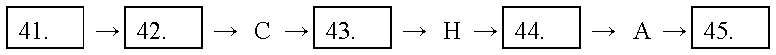
\includegraphics[width=\linewidth]{2025-01.assets/figure-012-004.pdf}\end{center}

\subsection*{\textbf{Part C}}


\subsection*{\textbf{Directions:}}


Read the following text carefully and then translate the underlined segments into Chinese. Write your answers on the ANSWER SHEET. (10 points)


Innovation and research have relied on public participation in science for centuries. It was a musician who discovered the planet Uranus in the 18th century by making his own telescope with mirrors composed of copper and tin. (46) \uline{Recent decades have seen science move into a} \uline{convention where engagement in the subject can only be done through institutions, such as a} \uline{university.} Citizen science provides an opportunity for greater public engagement and the democratisation of science.


In the information era, large data sets, small teams and financial restrictions have slowed scientific process. (47) \uline{But by utilising the natural curiosity of the general public it is possible to} \uline{overcome many of these challenges by engaging non-scientists directly in the research process.} Anyone can be a citizen scientist, regardless of age, nationality or academic experience. You don’t even need any formal training, just an inquisitive mind and the enthusiasm to join one of the thousands of citizen science projects to generate new knowledge and the means to understand a genuine scientific outcome.


(48) \uline{Scientists have employed a variety of ways to engage the general public in their research,} \uline{such as making data analysis into an online game or sample collection into a smartphone} \uline{application. }They’ve implored citizens to help with bug counting and categorising cancer cells, and even identifying distant galaxies.


This form of accessible science means that great minds are able to join the race to create and develop projects with the potential to change the world. A citizen science-based approach can extend the field of vision and include different ideas and different brains to problem-solve and create, making innovation faster and more effective.


The rise of citizen science has grown alongside the rise of do-it-yourself biology laboratories around the world. (49) \uline{These groups of people are part of a rapidly expanding biotechnological} \uline{social movement of citizen scientists and professional scientists seeking to take discovery out of} \uline{institutions and put it into the hands of anyone with the enthusiasm.}


There are around 40 official do-it-yourself biology centres across the globe in locations including Paris, London, Sydney, and Tel Aviv. (50) \uline{They pool resources, collaborate, think} \uline{outside the box, and find solutions and ways around obstacles to explore science for the sake of} \uline{science without the traditional boundaries of working inside a formal setting. }So is it time to take the Petri dish out of the laboratory and into the garage?


\subsection*{\textbf{Section III Writing}}


\subsection*{\textbf{Part A}}


\textbf{51. Directions:}


Read the following email from your classmate Paul and write him a reply.


Dear Li Ming, I was really excited to hear that you’d invite some young craftsmen to demonstrate their innovative craft-making on campus. May I know more about what they’ll Show? Also, I’d like to help with your preparation work. Please let me know what I can do.


Yours, Paul


Write your answer in about 100 words on the ANSWER SHEET. \textbf{Do not} use your own name in your email; use “Li Ming” instead. (10 points)


\subsection*{\textbf{Part B}}


\textbf{52. Directions:}


Write an essay of 160-200 based on the following table. In your essay, you should


1) describe the table briefly,


2) explain its intended meaning, and


3) give your comments.


You should write neatly on the ANSWER SHEET. (20 points)


\begin{center}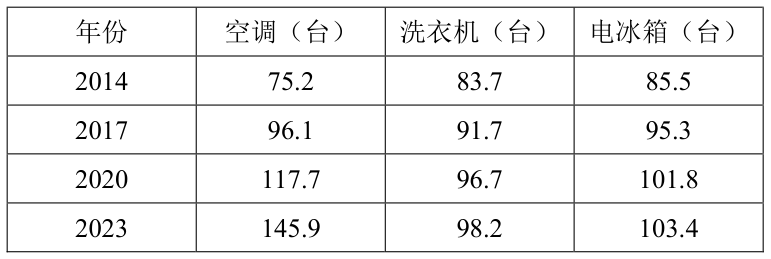
\includegraphics[width=.85\linewidth,height=.55\textheight,keepaspectratio]{2025-01.assets/figure-014-014.png}\end{center}

\begin{center}近年来全国居民平均每百户年末主要耐用消费品拥有量\end{center}
\end{document}